\section{Additional Results}
\label{app:results}
%
We provide additional evaluation of our method, following Section 5 of the main text.

In \autoref{tab:ssplats_benchmarks}, we provide an ablation study of an important variant of our algorithm. We replace the sorting-based forward pass with the stochastic algorithm in Algorithm 1 of the main paper, proposed by \citet{Sun2025}, vary the number of samples used in the forward pass and evaluate the performance on novel view synthesis tasks. Experiment shows that our hybrid approach consistently outperforms the full stochastic variants in terms of both reconstruction quality and time. 

\begin{table}[t]
    \centering
    \caption{
        NeRF Synthetic Dataset
    }
    \small
    \begin{tabular}{c|c c c c}
        \toprule
        & \textbf{PSNR$\uparrow$} & \textbf{SSIM$\uparrow$} & \textbf{LPIPS$\downarrow$} & \textbf{Time$\downarrow$}\\
        \midrule
        3DGRT & 33.84 & 0.970 & 0.038 & 10m21s \\
        SS-Tracing & 31.67 & 0.958 & 0.050 & 24m31s\\
        \textbf{Ours} & 33.99 & 0.970 & 0.039 & 6m57s\\
        \bottomrule
    \end{tabular}
    \label{tab:benchmark_nerf}
\end{table}

In \autoref{tab:benchmark_nerf}, we show the metrics of our method, 3DGRT and SS-Tracing on the NeRF-Synthetic dataset. Our performance is consistent with the results we show in the main paper.

\begin{figure}[t]
    \setlength{\resLen}{1.5in}
    %
    \centering
    \small
    \addtolength{\tabcolsep}{-5.5pt}
    %
    %
    \begin{tabular}{cc}
        % &
        (a) \textbf{Original} & (b) \textbf{Ours}
        \\
        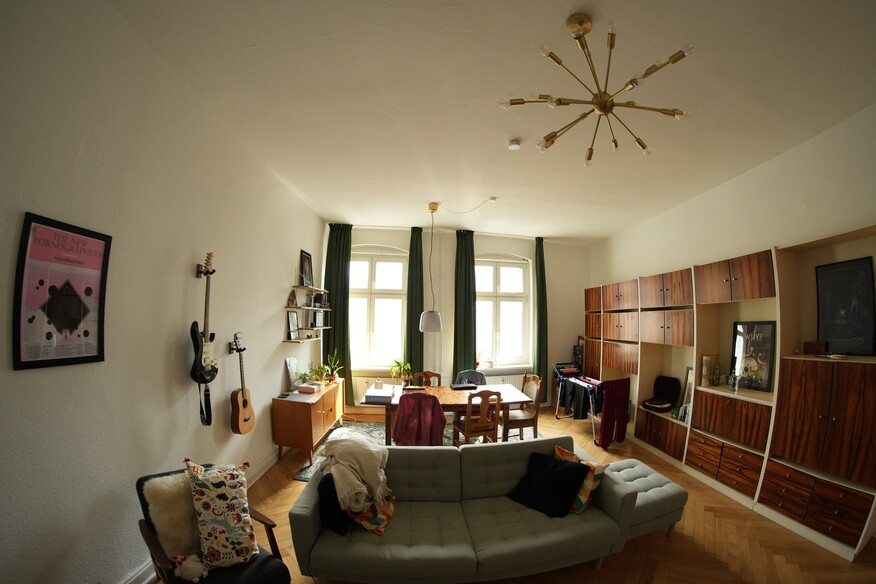
\includegraphics[width=\resLen]{images/fisheye/reference0.jpg} &
        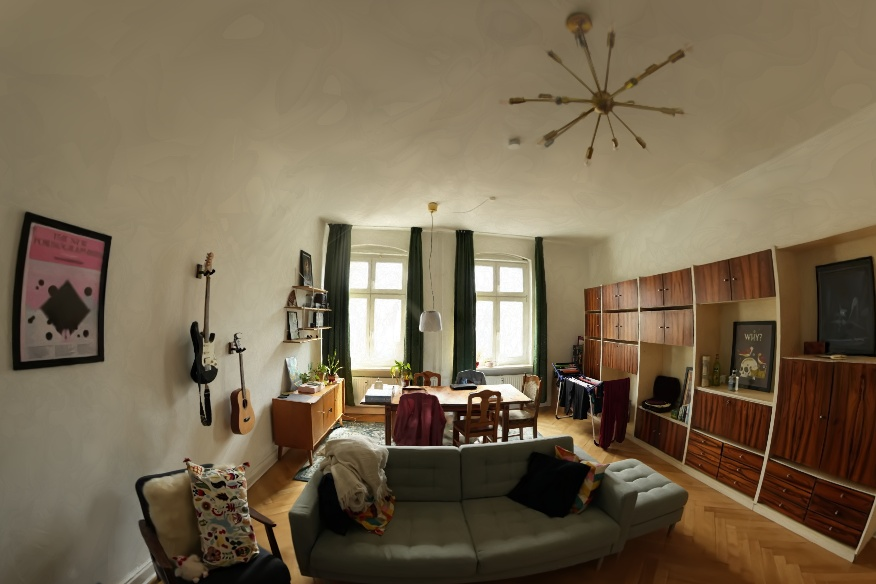
\includegraphics[width=\resLen]{images/fisheye/ours0.jpg} 
        \\
        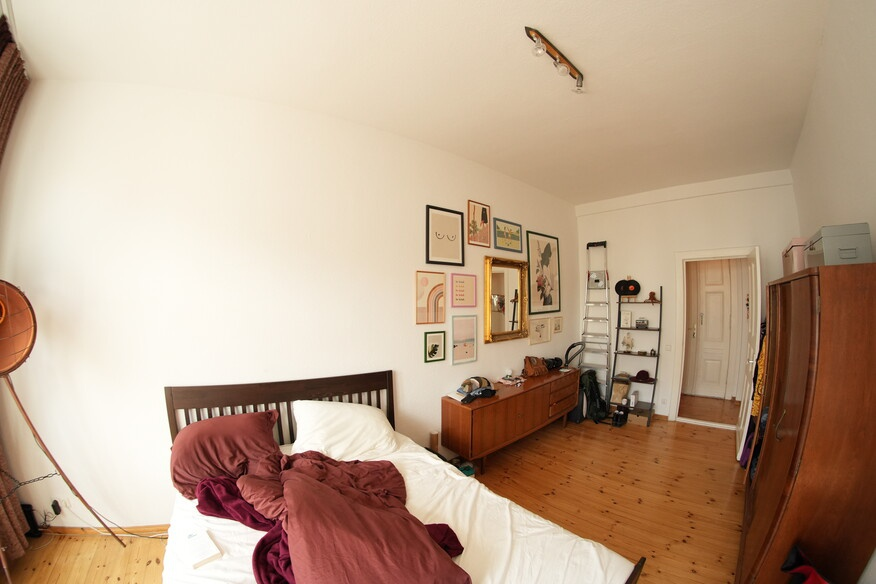
\includegraphics[width=\resLen]{images/fisheye/reference1.jpg} &
        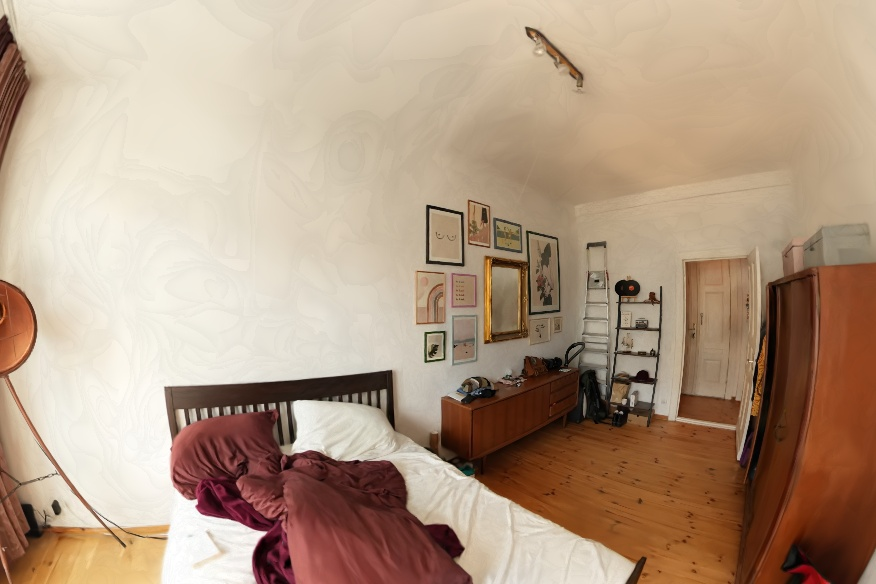
\includegraphics[width=\resLen]{images/fisheye/ours1.jpg}
    \end{tabular}
    %
    \caption{
        Similar to our ray tracing baseline, our method also seamlessly supports distorted cameras, e.g., fisheye.
    }
    \label{fig:fisheye}
\end{figure}

In \autoref{fig:fisheye}, we demonstrate that our method is seamlessly compatible with distorted camera models due to the usage of ray tracing.

In \autoref{fig:nvs_figures_more}, we show additional results of the equal-time novel view synthesis benchmark. In \autoref{fig:relightable_figures_more}, we show additional results from relightable Gaussian splatting evaluations. 

\begin{figure*}[t]
    \setlength{\resLen}{1.75in}
    %
    \centering
    \small
    \setlength{\tabcolsep}{1pt}
    \renewcommand{\arraystretch}{0}
    %
    %
    \begin{tabular}{cccc}
        % &
        \textbf{Reference} & (a) \textbf{Ours} & (b) \textbf{3DGS} & (c) \textbf{3DGRT}
        \\[3pt]
        
\includegraphics[width=\resLen]{images/equal-time/counter/reference_composite.jpg} &
        
\includegraphics[width=\resLen]{images/equal-time/counter/ours_composite.jpg} &
        
\includegraphics[width=\resLen]{images/equal-time/counter/3dgs_composite.jpg} &
        
\includegraphics[width=\resLen]{images/equal-time/counter/3dgrt_composite.jpg} 
        \\[3pt]
        
\includegraphics[width=\resLen]{images/equal-time/stump/reference_composite.jpg} &
        
\includegraphics[width=\resLen]{images/equal-time/stump/ours_composite.jpg} &
        
\includegraphics[width=\resLen]{images/equal-time/stump/3dgs_composite.jpg} &
        
\includegraphics[width=\resLen]{images/equal-time/stump/3dgrt_composite.jpg} 

    \end{tabular}
    %
    \caption{\textbf{Equal-time Comparison} between our method and baselines. We run the methods for the same period of wall-clock time, and compare the reconstruction quality. Our method produces comparable visual quality to 3DGS, and outperforms 3DGRT.
    }
    \label{fig:nvs_figures_more}
\end{figure*}


\begin{figure*}[t]
    \setlength{\resLen}{1.75in}
    %
    \centering
    \small
    \setlength{\tabcolsep}{1pt}
    \renewcommand{\arraystretch}{0}
    %
    %
    \begin{tabular}{cccc}
        % &
        \textbf{Reference} & (a) \textbf{Ours} & (b) \textbf{RNG} & (c) \textbf{GS$^3$}
        \\[3pt]
        
\includegraphics[width=\resLen]{images/relightable/lego/reference_composite.jpg} &
        
\includegraphics[width=\resLen]{images/relightable/lego/ours_composite.jpg} &
        
\includegraphics[width=\resLen]{images/relightable/lego/RNG_composite.jpg} &
        
\includegraphics[width=\resLen]{images/relightable/lego/GS3_composite.jpg}
        \\[2pt]
        
\includegraphics[width=\resLen]{images/relightable/furball/reference_composite.jpg} &
        
\includegraphics[width=\resLen]{images/relightable/furball/ours_composite.jpg} &
        
\includegraphics[width=\resLen]{images/relightable/furball/RNG_composite.jpg} &
        
\includegraphics[width=\resLen]{images/relightable/furball/GS3_composite.jpg}
        \\[2pt]
    \end{tabular}
    %
    \caption{Visualization of reconstruction quality of our method and baselines. Our method produces significantly better geometry, and in particular, shadow quality.
    }
    \label{fig:relightable_figures_more}
\end{figure*}
